\documentclass{sigchi-ext}
% Please be sure that you have the dependencies (i.e., additional
% LaTeX packages) to compile this example.
\usepackage[T1]{fontenc}
\usepackage{textcomp}
\usepackage[scaled=.92]{helvet} % for proper fonts
\usepackage{graphicx} % for EPS use the graphics package instead
\usepackage{balance}  % for useful for balancing the last columns
\usepackage{booktabs} % for pretty table rules
\usepackage{ccicons}  % for Creative Commons citation icons
\usepackage{ragged2e} % for tighter hyphenation

\usepackage{amsmath}
\usepackage{amsthm}
\usepackage{amssymb}
\graphicspath{{figures/}{./}}

% \usepackage{marginnote} \usepackage[shortlabels]{enumitem}
% \usepackage{paralist}

%% EXAMPLE BEGIN -- HOW TO OVERRIDE THE DEFAULT COPYRIGHT STRIP --
\copyrightinfo{Permission to make digital or hard copies of all or
 part of this work for personal or classroom use is granted without
 fee provided that copies are not made or distributed for profit or
 commercial advantage and that copies bear this notice and the full
 citation on the first page. Copyrights for components of this work
 owned by others than ACM must be honored. Abstracting with credit is
 permitted. To copy otherwise, or republish, to post on servers or to
 redistribute to lists, requires prior specific permission and/or a
 fee. Request permissions from permissions@acm.org.\\
 {\emph{CHI'14}}, April 26--May 1, 2014, Toronto, Canada. \\
 Copyright \copyright~2014 ACM ISBN/14/04...\$15.00. \\
 DOI string from ACM form confirmation}
%% EXAMPLE END

\title{Selecting scenarios in temporal ensembles}

\numberofauthors{6}
% Notice how author names are alternately typesetted to appear ordered
% in 2-column format; i.e., the first 4 autors on the first column and
% the other 4 auhors on the second column. Actually, it's up to you to
% strictly adhere to this author notation.
\author{%
  \alignauthor{%
    \textbf{Guilherme G. Schardong}\\
    \textbf{Simone D. J. Barbosa}\\
    \textbf{Waldemar Celes}\\
    \textbf{H\'{e}lio Lopes}\\
    \affaddr{Department of Informatics - PUC-Rio} \\
    \affaddr{Rua Marqu\^{e}s de S\~{a}o Vicente, 225, G\'{a}vea, Rio de Janeiro - RJ} \\
    \email{gschardong@inf.puc-rio.br} }\alignauthor{%
    \textbf{Regis Kruel Romeu}\\
    \textbf{Alexandre Emerick}\\
    \textbf{Luciano Reis}\\
    \textbf{Ricardo Chaves}\\
    \affaddr{PETROBRAS}\\
    \email{author5@anotherco.com} } }

% Paper metadata (use plain text, for PDF inclusion and later
% re-using, if desired)
\def\plaintitle{Selecting scenarios in temporal ensembles} \def\plainauthor{Guilherme G. Schardong, Simone D. J. Barbosa, Waldemar Celes, Regis Kruel Romeu, Alexandre Emerick, Luciano Reis, Ricardo Chaves and H\'{e}lio Lopes}
\def\plainkeywords{Representative Model Selection; Ensemble Methods; Time Series Processing; Brushing and Linking; Multidimensional Scaling.}
\def\plaingeneralterms{Ensemble Selection}

%% Set up our PDF with metadata
\hypersetup{%
  pdftitle={\plaintitle}, pdfauthor={\plainauthor},
  pdfkeywords={\plainkeywords}, }

% \reversemarginpar%

\begin{document}

\maketitle

% Uncomment to disable hyphenation (not recommended)
% https://twitter.com/anjirokhan/status/546046683331973120
\RaggedRight{} 

% Do not change the page size or page settings.
\begin{abstract}
  When dealing with large ensemble datasets, their sheer size may hinder any analysis necessary to extract knowledge from them. To solve this problem a number of selection approaches have been proposed. We propose an approach based on a score function for time series ensembles, along with a novel graphical tool, the rank chart, to evaluate a time series adherence to a reference series. We compare our results with a manual selection using a brushing and linking framework and with a $k$ Nearest Neighbors based selection of the series after projecting them using a Multidimensional Scaling algorithm. To evaluate our approach, we applied it to an oil reservoir ensemble in order to find the models with the best adherence to a set of reference time series. The results of our case study indicate that the proposed score function attained good results in the ranking of the time series and the rank chart proved to be an invaluable tool to analyze the behavior of the selected series compared to a reference set.
\end{abstract}

\keywords{\plainkeywords}

\category{G.3}{Probability and Statistics}{Time Series Analysis}

\section{Introduction}
The recent introduction of ensemble methods in the oil industry has made it possible to apply several newer computational approaches to solve existing problems, such as: history matching \cite{aanonsen:2009}, enhance production forecasts \cite{wen:2005}, and improve strategical planning for oil reservoirs \cite{aanonsen:2009, chen:2009}. One of the key tasks in reservoir management is to evaluate the profitability of a reservoir. To accomplish this, a production strategy is developed and simulated in order to estimate the ammount and flow of hydrocarbons in the field. Due to uncertainties inherent to the geological model, serveral hundred possible scenarios are obtained for each strategy.

Steagall and Schiozer \cite{steagall:2001} propose the use of three classes of models to evaluate the performance of a production strategy: a pessimistic, probable and optimistic models with respect to the Net Present Value (NPV). Schiozer et al. \cite{schiozer:2004} improved the approach by requiring that the models selected be representative in other properties, such as Cumulative Oil Production (NP), Cumulative Water Production (WP) and Oil Recovery Factor (ORF) as well.

However the process of selecting this subset is a challenging task due to the sheer number of possible outcomes of a simulation and the constraints that need to be satisfied. Several approaches have been proposed to accomplish this task, ranging from optimization based approaches, to clustering and classification. We propose an approach that takes into account a range of time from each simulation and rank its outcomes according to a score function detailed below. We also propose a novel time series visualization tool to help analyze the adherence of each series the a set of percentile curves (P$_{10}$, P$_{50}$ and P$_{90}$) calculated from the simulations, as proposed by Stegall and Schiozer \cite{steagall:2001}.

\section{Related Work}
\label{sec:rel-work}
The analysis and visualization of ensemble data is a daunting task due to their high complexity and dimensionality. As a result, there are several published approaches to accomplish these tasks \cite{phadke:2012, hlawitschka:2013, ensemblevis-potter:2009, multicharts-demir:2014}. In particular, Potter et al. \cite{ensemblevis-potter:2009} proposed the development of a framework for statistical visualization of bidimensional weather ensembles. The work of Demir et al. \cite{multicharts-demir:2014} proposed a technique for the interactive visual exploration of tridimensional scalar ensembles using brushing and linking, in addition to line and bar charts of statistical data measures.

Another approach to analyze this data is to select a reduced number of elements that are representative of the whole ensemble. Recent approaches have modelled this task as an optimization problem, where the goal is to maximize, or minimize, an objective function. In this context, Sarma et al. \cite{selection-sarma:2013} modeled the selection as a constrained minimax combinatorial optimization problem and solved it by doing an exhaustive search over the solution space for small ensembles and by employing a greedy algorithm to search for a solution in larger ensembles. Their approach reportedly performs faster and is more accurate than clustering approaches. Meira et al. \cite{meira:2016} employed the same approach to select a set of representative models that minimizes a multi-objective cost function composed by a risk curve factor, an attribute-level coverage factor and a weighted cross plot spread factor. By minimizing this function, Meira's approach selects high quality sets of representative models without optimistic or pessimistic biases. Both approaches show that the optimization approach obtains promising results while maintaining a good computational cost.

\section{Tools and Techniques}
\label{sec:tools}
This section describes the techniques developed in our work.

\subsection{Objective Function}
\label{sec:obj_func}
In order to select the representative models, we must define the criteria they must satisfy. The desired models must be close to a set of reference models selected by the user. The traditional approach uses the P$_{10}$, P$_{50}$ and P$_{90}$ models calculated from the ensemble as references. Given the absolute ranking calculated based on the euclidean distance between the entities, we assign a score for each possible rank. For an ensemble of $N$ entities, we use a linear function $f(r) = N - r - 1$, where $\left(r \in \mathbb{N} | r \in [1, N] \right)$ as the score for each rank $r$. We also assign a weight for each simulation time step based on the desired adherence between the candidate models and the references. The definition of this function depends on the type of analysis and behavior of the ensemble itself.

\subsection{Rank Chart}
\label{sec:rank}
When searching for meaningful entities in an ensemble there is usually a synthetic ideal entity used as reference, and the task is to select the ensemble entity that most closely resembles the reference. With time series data, the user may search for a series that closely matches the reference in a number of time steps. To help with this task, a novel type of visualization is proposed: the Rank Chart. This chart graphs the ranking of ensemble elements against a reference, along the time axis. Figure \ref{fig:rank-sample} shows an example of a rank chart.

The rank chart is built by iterating through the time steps of the ensemble entities and calculating the distance between each series and the reference up to that step. This distance is then ordered in ascending order and ranked accordingly. This process creates a new set of time series, now composed of the absolute ranks attained by each ensemble entity at each time step. These ranks are then plotted in a two-dimensional plane where the $X$ axis is the time step and the $Y$ axis is the rank.

\begin{figure}
  \centering
  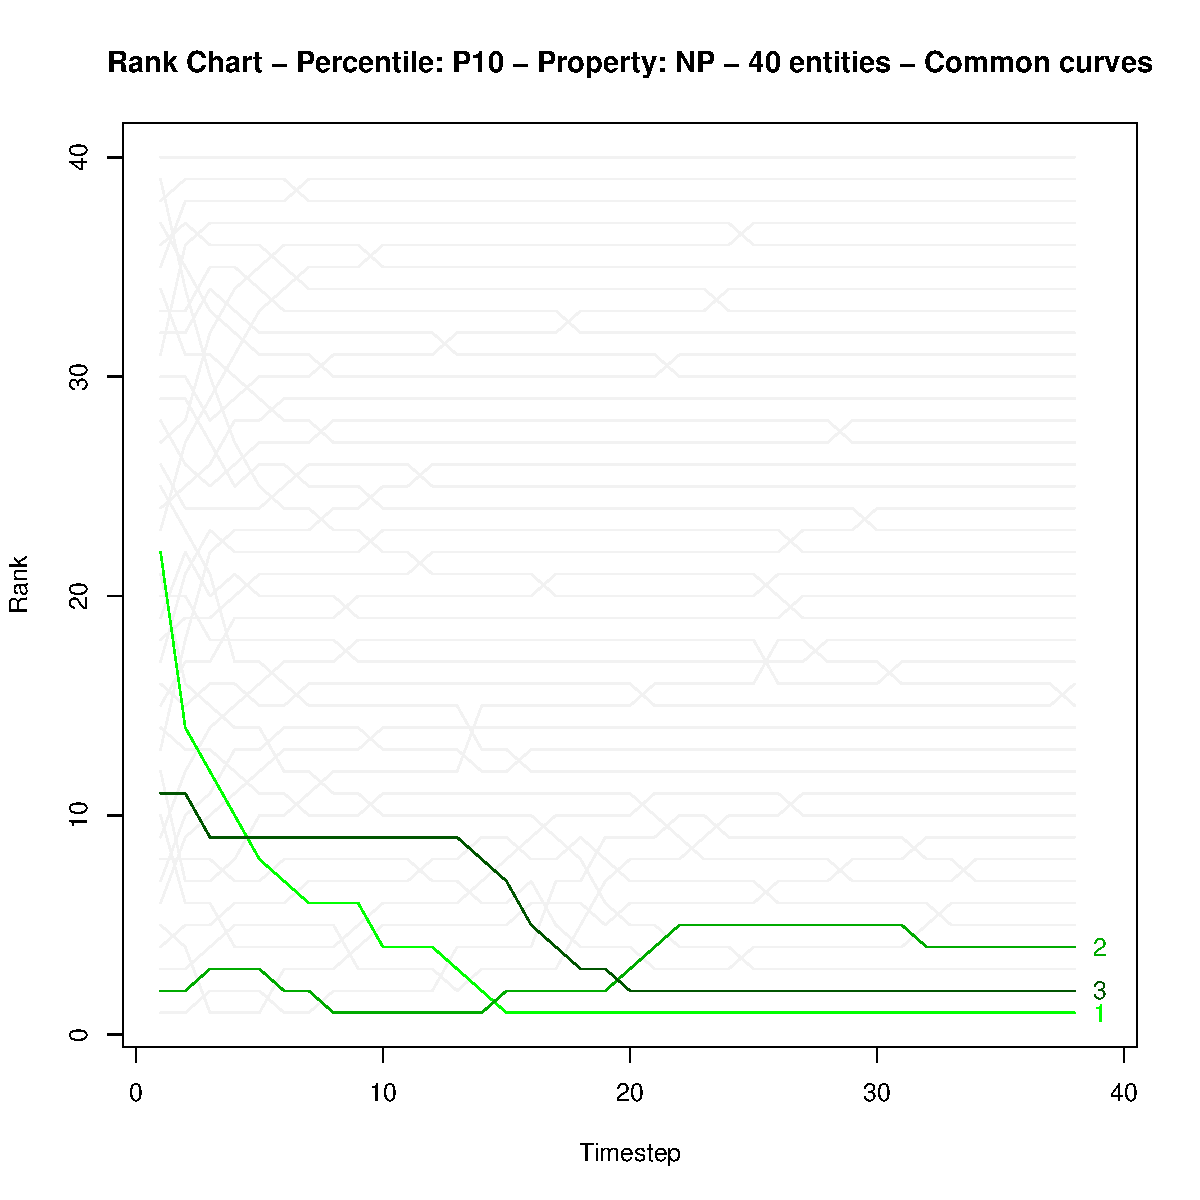
\includegraphics[width=0.7\columnwidth]{rank-common-40.pdf}
  \caption{Rank chart of 40 ensemble elements using the calculated P$_{10}$ curve as reference. The curves in green were selected by both the score and manual approaches.}
  \label{fig:rank-sample}
\end{figure}

\section{Experiments}
\label{sec:experiments}
As a proof of concept, the techniques presented in this work have been applied using simulations of a synthetic oil reservoir. The data are composed of 200 simulations before and after history matching. Each simulation possesses several properties of varied types, such as grid porosity, permeability and oil, water and gas saturations, as well as fluid productions of each reservoir well.

One of the key analysis tasks is the selection of the P$_{10}$, P$_{50}$ and P$_{90}$ models based on the production forecast data. These models can be used to compare the performance of different strategies applied on the same reservoir.

The process begins with the selection of the wells and properties to be processed. For our analysis, we selected the cumulative oil production (NP) of the producer wells. The score weight function chosen is the $w(t) = arctan(t)$. The first set of candidates was selected using a score based approach. The second set was selected manually using a scatter chart with the models in the $x$ axis and their distance to the reference in the $y$ axis. The third set of models was selected by applying a $k$ Nearest Neighbors on the projections of the models after applying a Multidimensional Scaling (MDS) algorithm. Figure \ref{fig:models-p50} shows rank and fan charts of the candidates for each approach in the P$_{50}$ case.

\begin{figure}
  \centering
  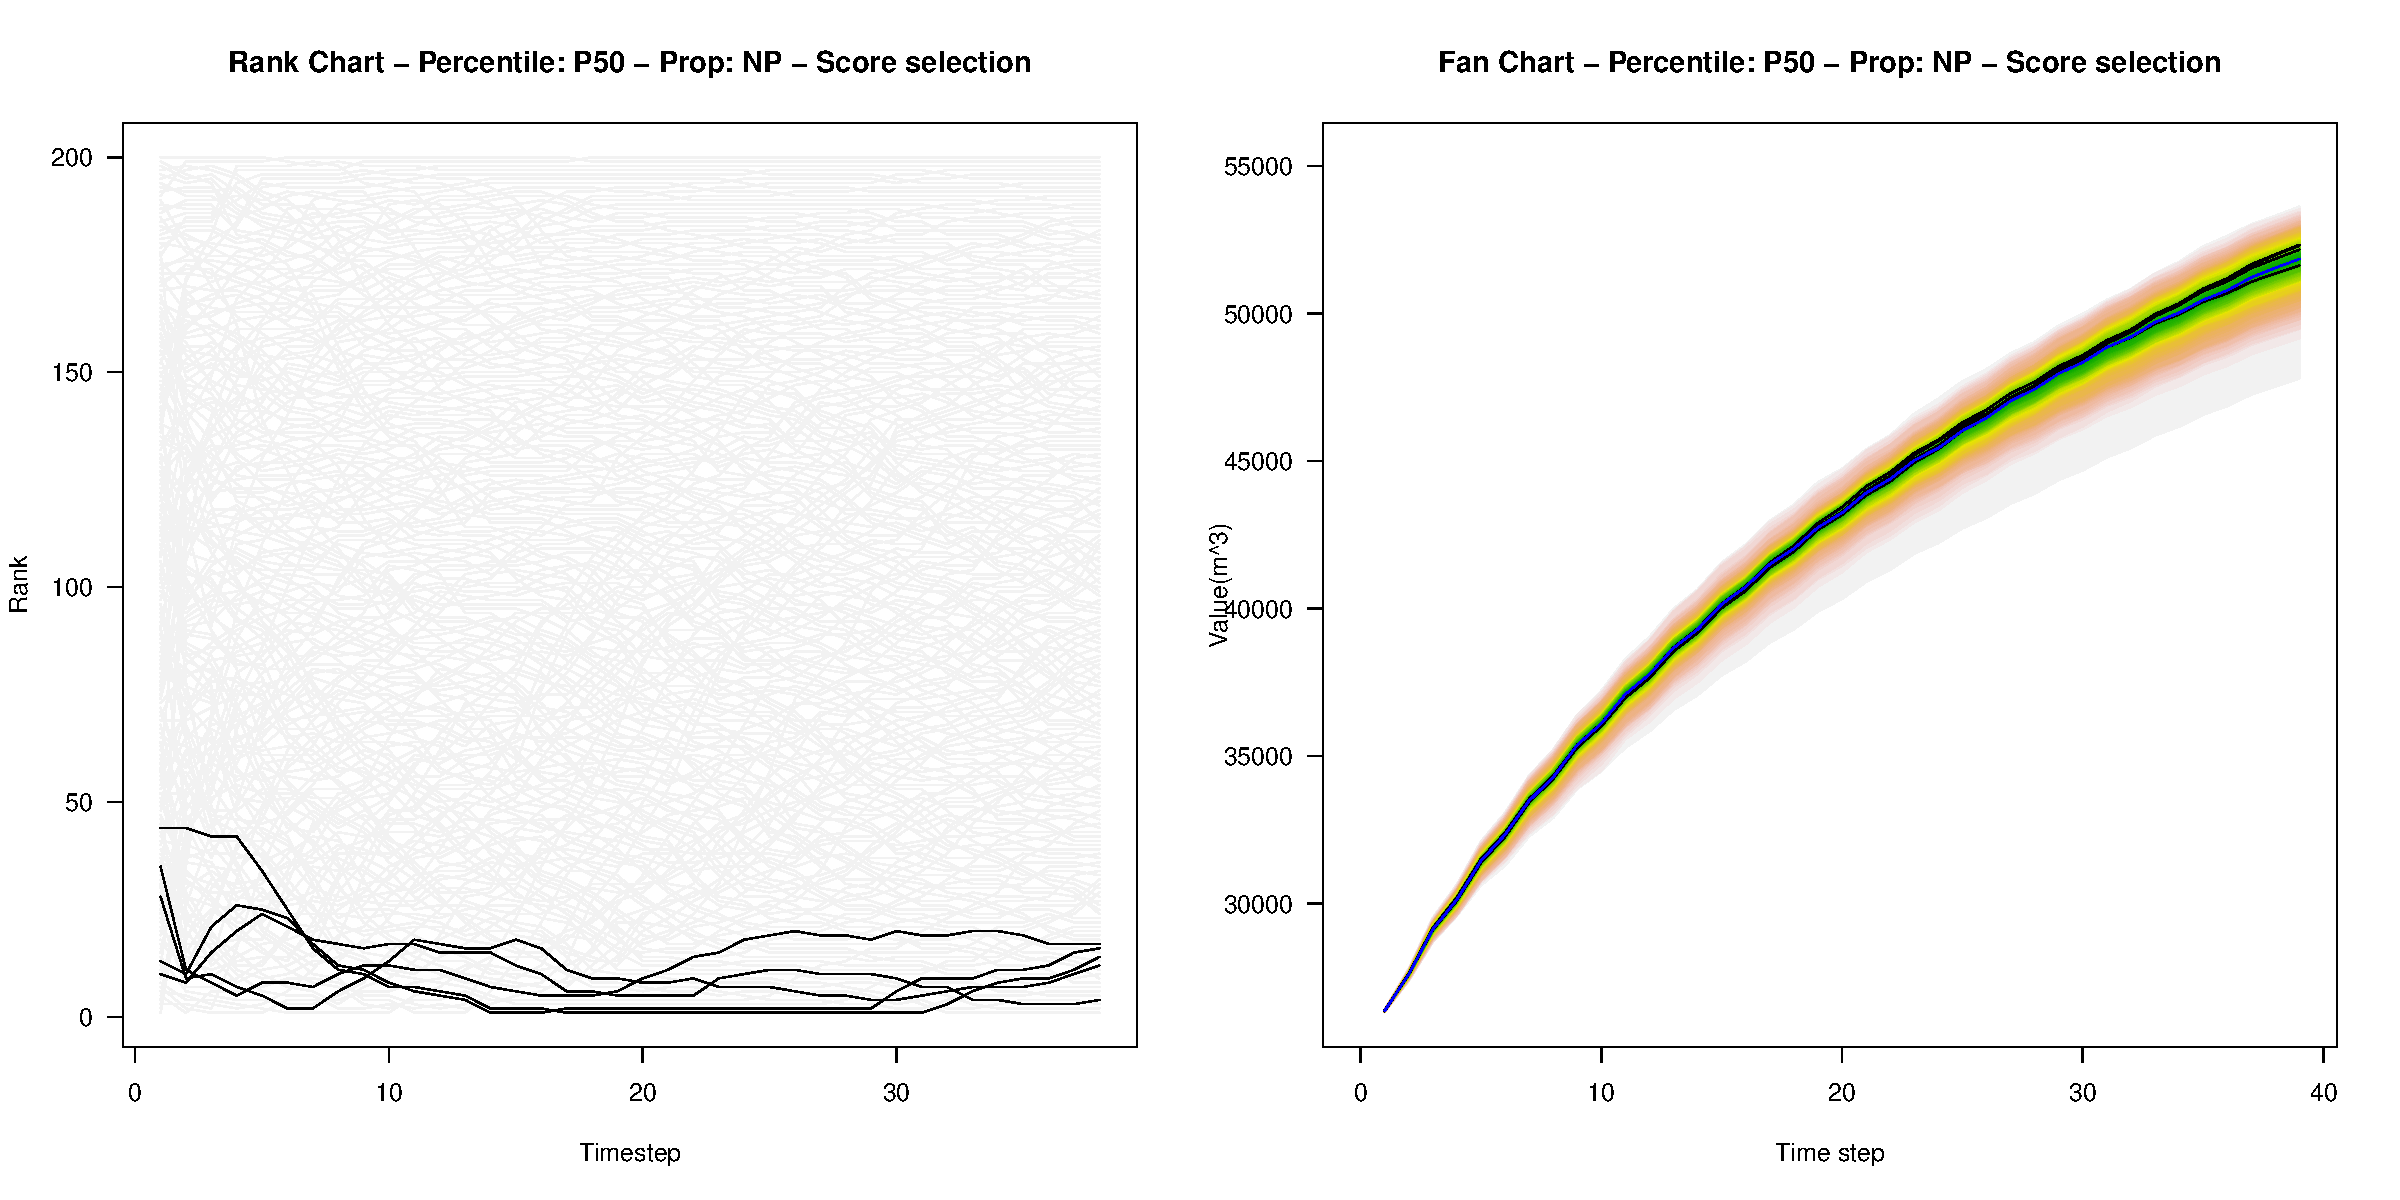
\includegraphics[width=\columnwidth]{rank-fan-score-p50.pdf}
  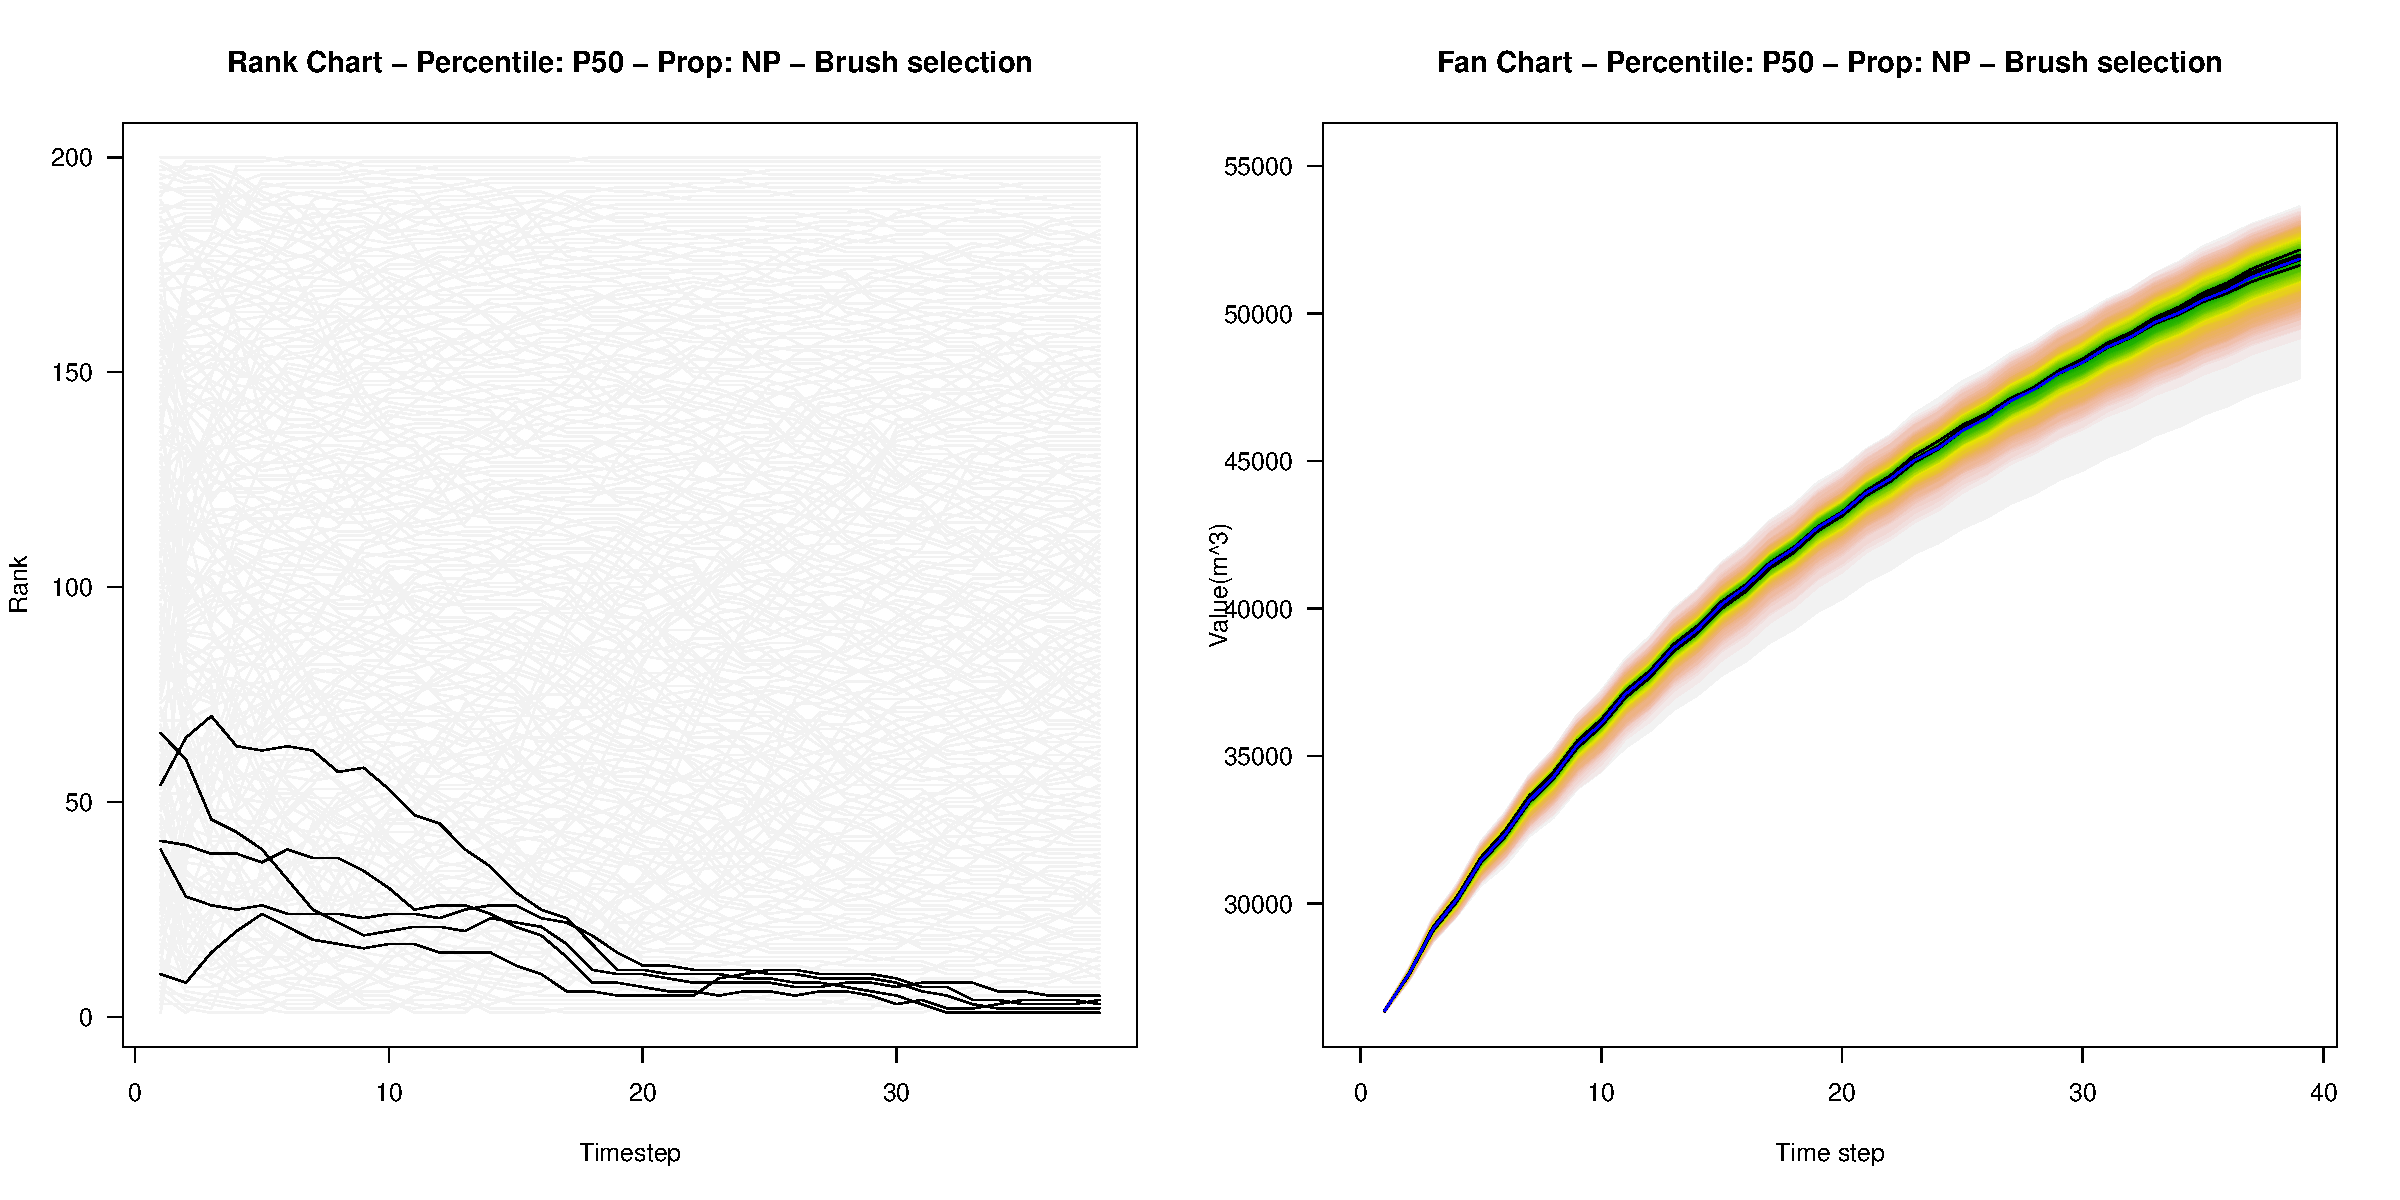
\includegraphics[width=\columnwidth]{rank-fan-brush-p50.pdf}
  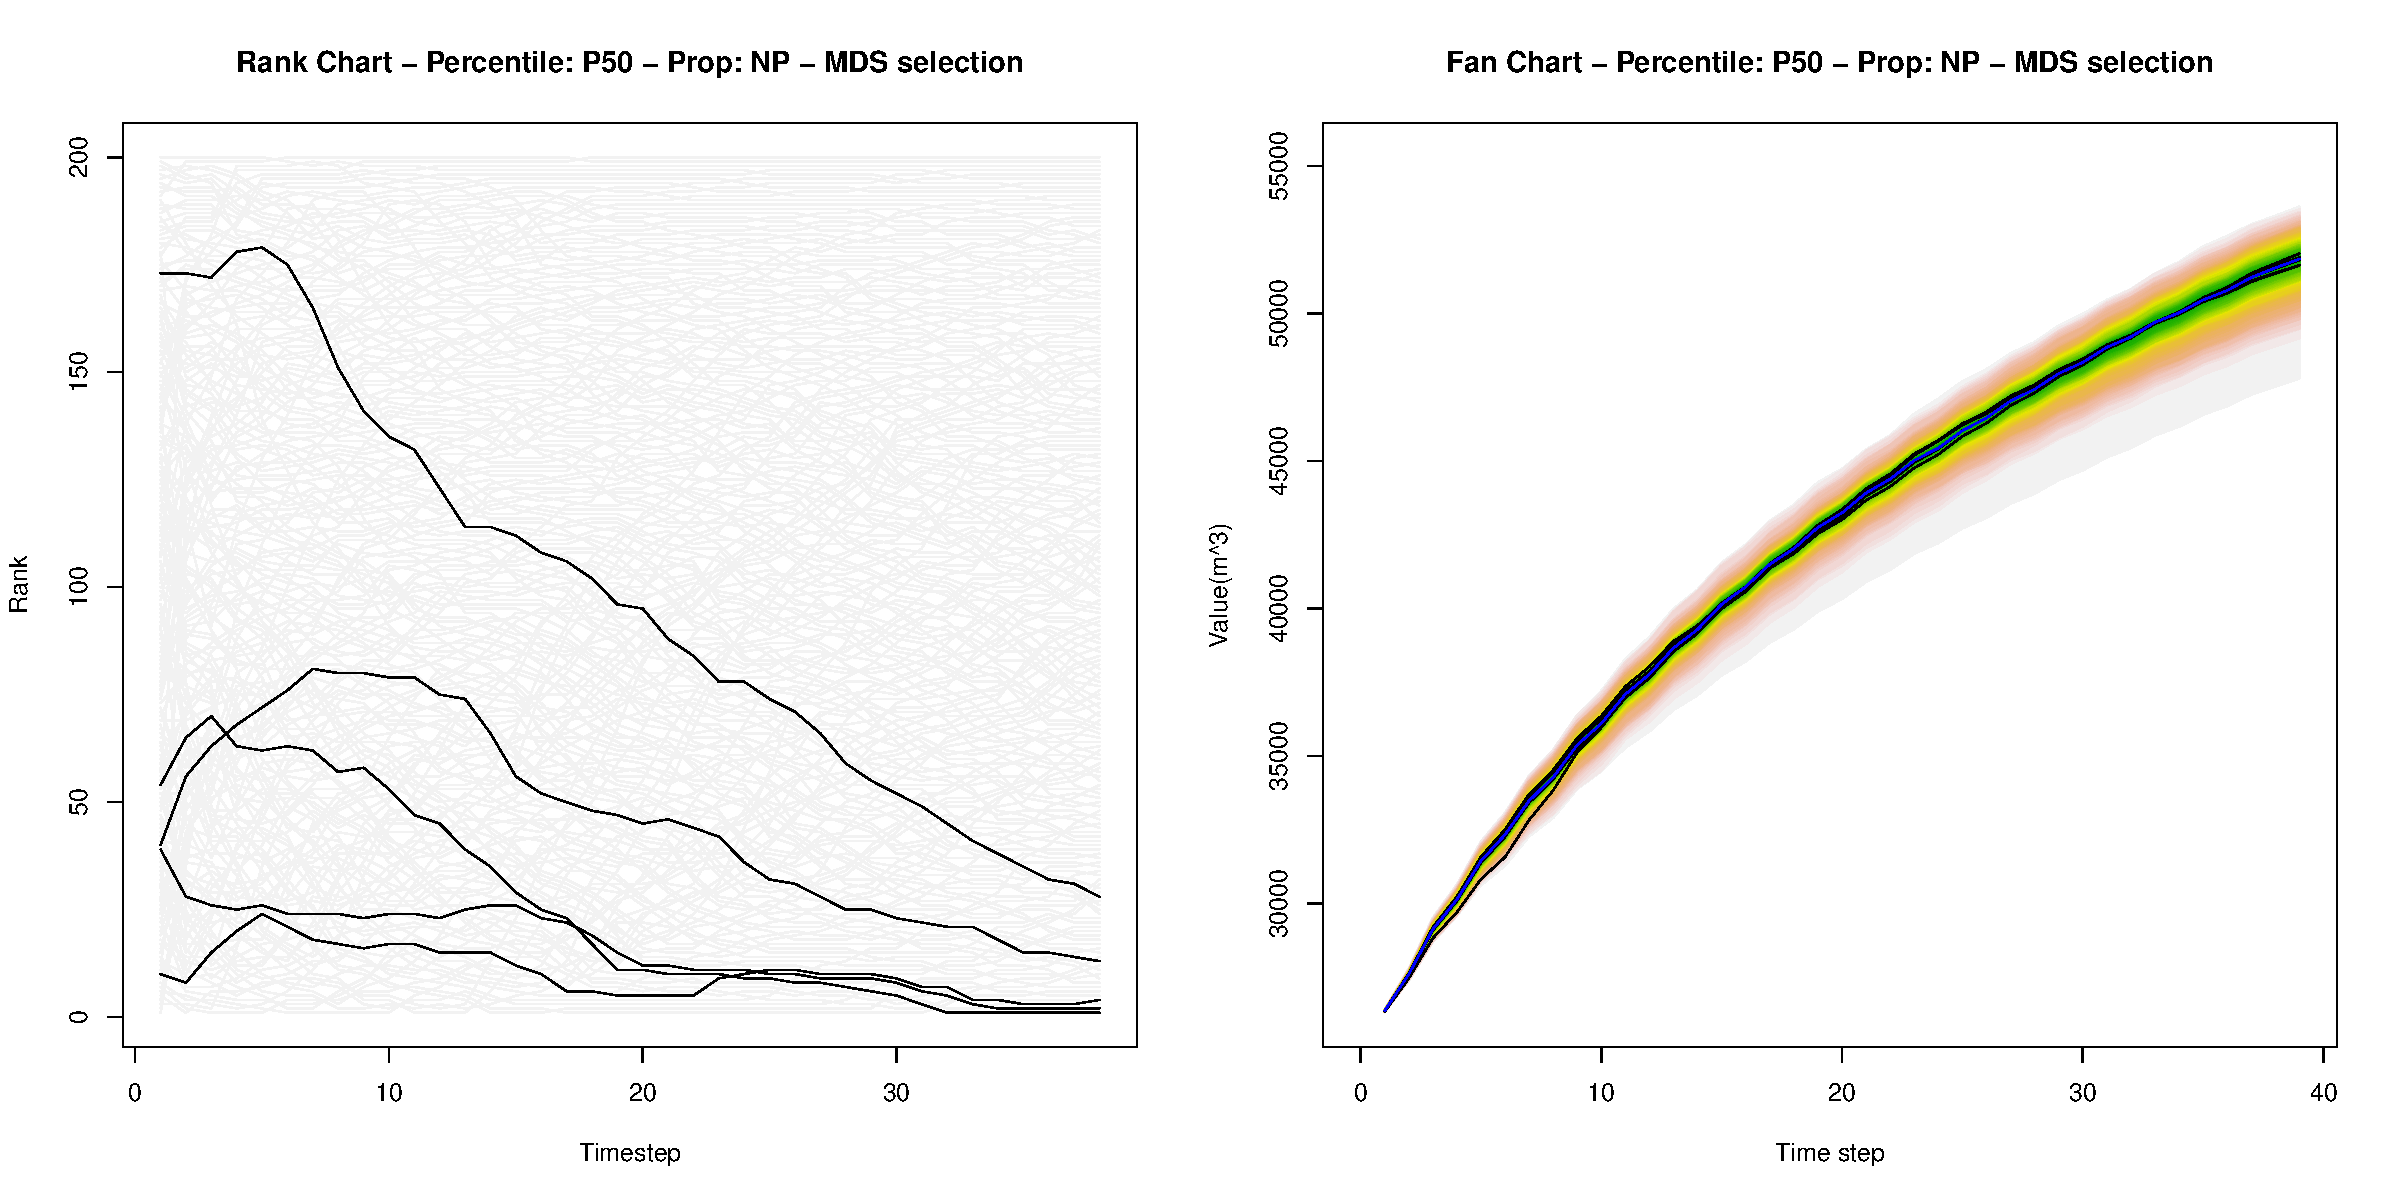
\includegraphics[width=\columnwidth]{rank-fan-mds-sel-p50.pdf}
  \caption{Rank and Fan charts of the models selected by each approach for the P$_{50}$ percentile. From top to bottom, we have the score selection, manual selection and MDS kNN selection.}
  \label{fig:models-p50}
\end{figure}

\section{Conclusions}
\label{sec:conclusion}
In this paper, we proposed an approach to select representative models for time series ensembles. To accomplish this task, we proposed a score function to automatically select a subset of time series as possible candidates for the representative model subset. The results indicate that our approach obtains a good set of possible candidates.

We also developed a graphical tool, named rank chart, in order to evaluate the adherence of ensemble members to a reference curve. When compared to other graphical tools, such as the fan chart, the behavior of the ensemble time series could be easily compared to a reference curve even in the presence of a low variance between the curves.

When compared to previous works, our approach makes a significant contribution by dealing with a range of production values. However, our approach considers only one property at a time. This may result in a sub-optimal selection when compared to more recent approaches \cite{selection-sarma:2013, meira:2016} which take into account multiple properties.

\balance{} 

% \bibliographystyle{ACM-Reference-Format-Journals}
\bibliographystyle{SIGCHI-Reference-Format}
% \bibliographystyle{acm}
\bibliography{references}

\end{document}

%%% Local Variables:
%%% mode: latex
%%% TeX-master: t
%%% End:
